\chapter{Grundlagen}\label{chap:grundlagen}

Dieses Kapitel stellt das theoretische Fundament der späteren praktischen Arbeit vor. Zunächst werden die
mathematischen und algorithmischen Grundlagen der Computertomographie erläutert, bevor die \gls{cuda}-Plattform als
technische Basis eingeführt wird.

\section{Die Computertomographie}

\subsection{Mathematische Grundlagen der Computertomographie}

In diesem Abschnitt werden die mathematischen Grundlagen der Computertomographie behandelt. Es werden zunächst die
mathematischen Eigenschaften der Vorwärtsprojektion und das sich daraus ergebende Fourier-Schichten-Theorem erläutert.
Anschließend wird die Aufnahme der Projektionen mit Parallelstrahlen erklärt und die Aufnahme mit Fächerstrahlen
abgeleitet. Zum Schluss wird das Prinzip der Fächerstrahlen auf den dreidimensionalen Raum ausgeweitet, also auf die
Aufnahme mit Kegelstrahlen.

\subsubsection{Projektionen}

Schießt man einen Röntgenstrahl durch ein festes Objekt, wie beispielsweise biologisches Gewebe oder ein Metall, so wird
dieser Strahl je nach Dichte des Materials entlang seiner Bahn abgeschwächt bzw.\ absorbiert. Mathematisch lässt sich
ein Objekt als zwei- oder dreidimensionale Verteilung von Absorptionskonstanten verstehen, während die gesamte
Abschwächung entlang einer Strahlbahn als Kurvenintegral dargestellt werden kann.

Die Grundlage der folgenden Ausführungen ist die Abbildung~\ref{fig:math_proj}. Als Beispiel dienen ein Objekt, hier als
die Funktion $f(x, y)$, sowie Kurvenintegrale, hier das Parameterpaar $(\alpha, t)$. Die Linie $AB$ lässt sich dann
durch die folgende Formel darstellen:

\begin{equation*}
    x \cdot \cos \theta + y \cdot \sin \theta  = t_1
\end{equation*}

oder allgemein für beliebige, zu $AB$ parallele, Linien:

\begin{equation}\label{eq:proj_obj}
    x \cdot \cos \theta + y \cdot \sin \theta = t
\end{equation}

\begin{figure}[!htb]
\centering
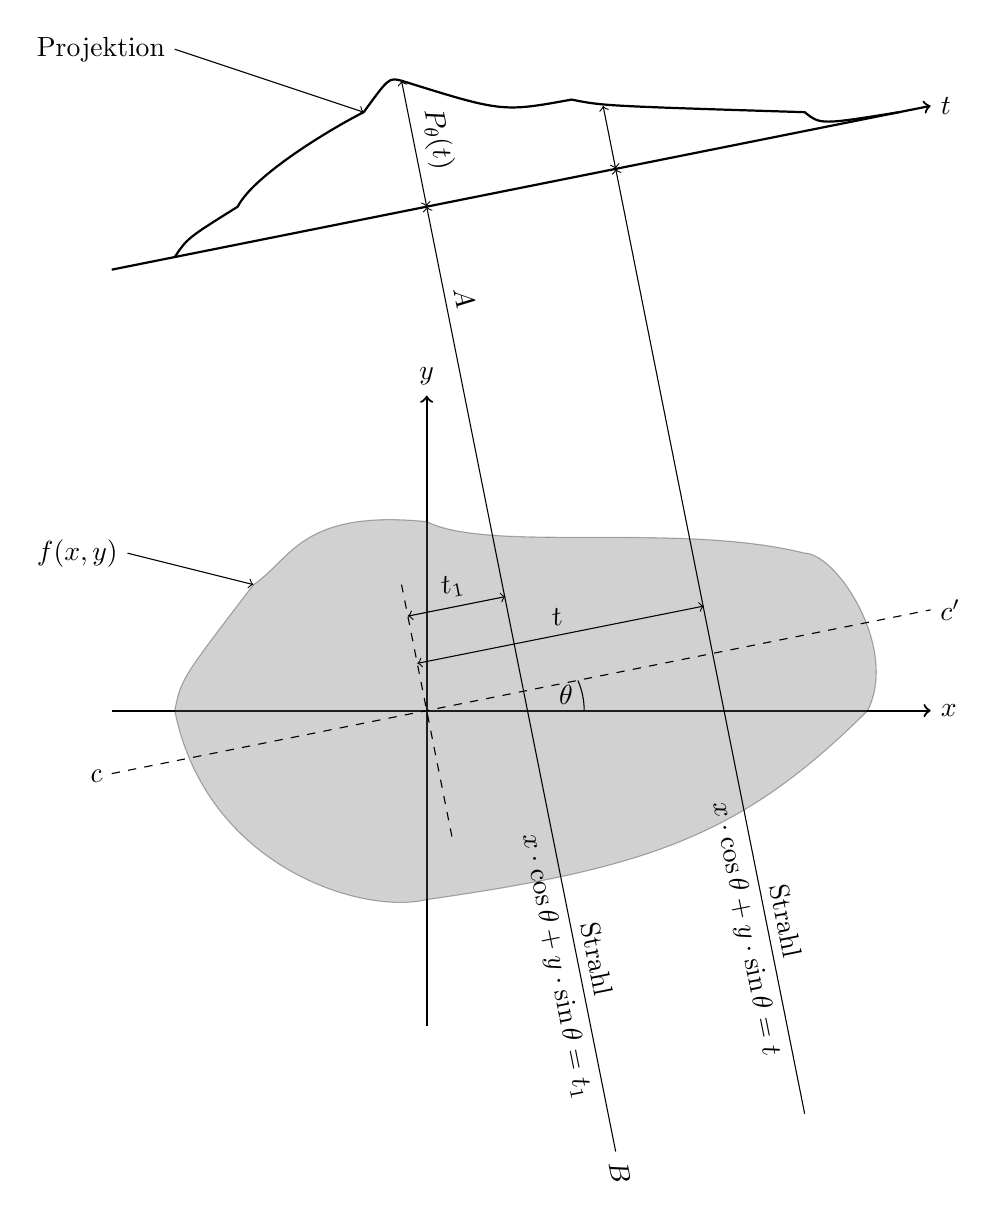
\begin{tikzpicture}[
    scale=0.8,
    axis/.style={thick,->}]
    % Achsen
    \draw[axis] (-5, 0) -- (8, 0) node[right] {$x$};
    \draw[axis] (0, -5) -- (0, 5) node[above] {$y$};
    \draw[axis] (-5, 7) -- (8, 9.6) node[right,sloped] {$t$};

    % Objekt
    \draw[fill=black!60!white,opacity=0.3] (0, -3) .. controls (3.5, -2.5) and (5, -2) .. (7, 0)
                                            .. controls (7.5, 1) and (6.5, 2.5) .. (6, 2.5)
                                            .. controls (4, 3) and (1, 2.5) .. (0,3)
                                            .. controls (-2, 3.2) and (-2.15, 2.4) .. (-2.75, 2)
                                            .. controls (-3.9, 0.5) .. (-4, 0)
                                            .. controls (-3.5, -2.5)  and (-1, -3.25) .. (0, -3);

    % Strahlen
    \draw[->] (3, -7) -- (0, 8) node[pos=0.9,above,sloped] {$A$} node[pos=0.2,above,sloped] {Strahl}
              node[pos=0.2,below,sloped] {$x \cdot \cos \theta + y \cdot \sin \theta = t_1$}
              node[pos=0,right,sloped] {$B$};

    \draw[->] (6, -6.4) -- (3, 8.6) node[pos=0.2,above,sloped] {Strahl}
              node[pos=0.2,below,sloped] {$x \cdot \cos \theta + y \cdot \sin \theta = t$};

    % t
    \draw[<->] (-0.3, 1.5) -- (1.25, 1.81) node[pos=0.5,above,sloped] {$t_1$};
    \draw[<->] (-0.15, 0.75) -- (4.4, 1.66) node[pos=0.5,above,sloped] {$t$};

    % sonstiges
    \draw[dashed] (-5, -1) -- (8, 1.6) node[pos=0,sloped,left] {$c$} node[sloped,right] {$c'$};
    \draw[dashed] (0.4, -2) -- (-0.4, 2);

    % Projektion
    \draw[<->] (0, 8) -- (-0.4, 10) node[pos=0.5, sloped, above] {$P_{\theta}(t)$};
    \draw[<->] (3, 8.6) -- (2.8, 9.6);
    \draw[thick] (-4, 7.2) .. controls (-3.8, 7.5) .. (-3, 8)
                 .. controls (-2.75, 8.5) and (-1.5, 9.25) .. (-1, 9.5)
                 .. controls (-0.6, 10.05) .. (-0.4, 10)
                 .. controls (1.2, 9.5) .. (2.3, 9.7)
                 .. controls (2.8, 9.6) .. (6, 9.5)
                 .. controls (6.25, 9.3) .. (7.5, 9.5);

    % Beschriftungen
    \draw[->] (-4.75, 2.5) -- (-2.75, 2) node[pos=0,left] {$f(x, y)$};
    \draw[->] (-4, 10.5) -- (-1, 9.5) node[pos=0, left] {Projektion};

    % Winkel
    \draw (2.5, 0) arc (0:23.5:12mm) node[pos=0.5,left] {$\theta$};
\end{tikzpicture}
\caption{Zusammenhang zwischen Kurvenintegral und Projektion (Vorlage:~\cite{kak79})}
\label{fig:math_proj}
\end{figure}

Das zu $f(x, y)$ gehörige Kurvenintegral ist $P_{\theta}(t)$:

\begin{equation}\label{eq:proj_int}
    P_{\theta}(t) = \int\limits_{(\theta, t)\text{-Linie}} f(x, y)\ \mathrm{d}s
\end{equation}

Zusammen mit der aus Formel~\ref{eq:proj_obj} resultierenden Delta-Distribution lässt sich das Kurvenintegral wie folgt
umschreiben:

\begin{equation}\label{eq:proj_radon}
    P_{\theta}(t) = \int\limits_{-\infty}^{\infty}\int\limits_{-\infty}^{\infty}f(x, y) \cdot \delta(x \cdot
                    \cos \theta + y \cdot \sin \theta - t)\ \mathrm{d} x\ \mathrm{d} y
\end{equation}

Die Funktion $P_{\theta}(t)$ ist die \textit{Radon-Transformation} der Funktion $f(x, y)$ (vgl.~\cite{radon}).

Eine Projektion lässt sich als die Kombination einer Menge von Radon-Transformationen verstehen. Die
(mathematisch) einfachste Projektion ist eine Sammlung von Parallelstrahlintegralen $P_{\theta}(t)$ unter einem
konstanten Winkel $\theta$. Man bezeichnet eine solche Projektion als \textit{Parallelstrahlprojektion} (siehe
Abbildung~\ref{fig:par_proj}). In der Praxis kann eine Parallelstrahlprojektion durch die Bewegung einer
Quelle-Detektor-Anordnung entlang paralleler Linien auf entgegengesetzten Seiten des Objekts aufgenommen werden.

Eine zweite Aufnahmemöglichkeit ist der Einsatz einer Quelle auf einer festen Position sowie einer Reihe von Detektoren
entlang einer Linie auf der anderen Seite des Objekts (siehe Abbildung~\ref{fig:fan_proj}). Solcherart erzeugte
Projektionen nennt man aufgrund der fächerförmigen Strahlen \textit{Fächerstrahlprojektionen} (vgl.~\cite{kakslan}).

\subsubsection{Das Fourier-Scheiben-Theorem}

Der Zusammenhang zwischen der Projektion und dem Objekt wird noch deutlicher, wenn man erstere einer eindimensionalen
und letztere einer zweidimensionalen Fouriertransformation unterzieht. So stellt Kak in seiner Arbeit fest, dass die
Fouriertransformation einer Parallelstrahlprojektion eines Objekts $f(x, y)$, die unter dem Winkel $\theta$
aufgenommen wurde, einer Schicht des zweidimensional fouriertransformierten Objekts $F(u, v)$, entspricht. Mit anderen
Worten ergibt die Fouriertransformation einer Projektion $P_{\theta}(t)$ die Werte von $F(u, v$) für ein bestimmtes
$v$(vgl.~\cite{kak85}).

Gemeinsam mit Slaney hat Kak diesen Zusammenhang mathematisch hergeleitet. Seien $F(u, v)$ die
zweidimensionale Fouriertransformation des Objekts $f(x, y)$:

\begin{equation}\label{eq:obj_2d_full}
    F(u, v) = \int\limits_{-\infty}^{\infty} \int\limits_{-\infty}^{\infty} f(x, y) \cdot e^{-2 \pi i \cdot(u x + v y)}\
        \mathrm{d} x\ \mathrm{d} y
\end{equation}

und $S_{\theta}(w)$ die eindimensionale Fouriertransformation der Projektion unter dem Winkel $\theta$ $P_{\theta}(t)$:

\begin{equation}\label{eq:proj_fft}
    S_{\theta}(w) = \int\limits_{-\infty}^{\infty} P_{\theta}(t) \cdot e^{-2 \pi i \cdot w t}\ \mathrm{d} t
\end{equation}

Im Folgenden sei der Fall $\theta = 0$ betrachtet. Setzt man $v = 0$, so wird die Formel~\ref{eq:obj_2d_full}
vereinfacht:

\begin{equation}
    F(u, 0) = \int\limits_{-\infty}^{\infty} \int\limits_{-\infty}^{\infty} f(x, y) \cdot e^{-2 \pi i \cdot u x}\
    \mathrm{d} x\ \mathrm{d} y
\end{equation}

Der Phasenfaktor ist nun nicht mehr von $y$ abhängig, wodurch das Integral in zwei Hälften geteilt werden kann:

\begin{equation}\label{eq:obj_2d_split}
    F(u, 0) = \int\limits_{-\infty}^{\infty} \left[\int\limits_{-\infty}^{\infty} f(x, y)\ \mathrm{d} y \right] \cdot
    e^{-2 \pi i \cdot u x}\ \mathrm{d} x
\end{equation}

Der Term in eckigen Klammern entspricht der Gleichung für eine Projektion entlang konstanter $x$-Linien:

\begin{equation}
    P_{\theta = 0}(x) = \int\limits_{-\infty}^{\infty} f(x, y)\ \mathrm{d} y
\end{equation}

Durch Einsetzen in Gleichung~\ref{eq:obj_2d_split} erhält man:

\begin{equation}
    F(u, 0) = \int\limits_{-\infty}^{\infty} P_{\theta = 0}(x) \cdot e^{-2 \pi i \cdot u x}\ \mathrm{d} x
\end{equation}

Die rechte Seite dieser Gleichung stellt die eindimensional fouriertransformierte Projektion $P_{\theta = 0}$ dar (vgl.
Gleichung~\ref{eq:proj_fft}), es ergibt sich also der folgende Zusammenhang zwischen der Projektion und dem
zweidimensional fouriertransformierten Objekt:

\begin{equation}
    F(u, 0) = S_{\theta = 0}(u)
\end{equation}

Dieses Ergebnis ist die einfachste Form des Fourier-Scheiben-Theorems. Darüber hinaus ist es unabhängig von der
konkreten Konstellation zwischen dem Objekt und dem Koordinatensystem der Projektion. Wird das
$(t, s)$-Koordinatensystem um den Winkel $\theta$ rotiert, so ist die Fouriertransformation der Projektion gleich der
zweidimensionalen Fouriertransformation des Objekts entlang einer radialen Linie, die um den Winkel $\theta$ rotiert
wird (siehe Abbildung~\ref{fig:fourier_scheibe}, vgl.~\cite{kakslan}).

\subsubsection{Parallelstrahlen}

\subsubsection{Fächerstrahlen}

\subsubsection{Kegelstrahlen}

\subsection{Die prinzipielle Funktionsweise der Computertomographie}

Am Anfang der Computertomographie steht das Röntgenverfahren, das 1895 vom deutschen Physiker Wilhelm Conrad Röntgen
entdeckt wurde~\cite{roentgen}. Mit Hilfe einer Strahlungsquelle wird ein Objekt durchleuchtet und auf einem Film bzw.\
einem Detektor abgebildet; der dreidimensionale Körper wird also auf eine zweidimensionale Fläche projiziert. Diesen
Schritt bezeichnet man als \textit{Vorwärtsprojektion}.

Führt man die Vorwärtsprojektion genügend oft in aufeinanderfolgenden Winkelschritten aus, bis man (idealerweise) einen
Vollkreis abgefahren hat, so lässt sich aus den dabei entstandenen \textit{Projektionen} der ursprünglich durchleuchtete
Körper, den wir in der Folge als \textit{Volumen} bezeichnen, rekonstruieren. Für jeden Punkt im Volumen
(\textit{\gls{voxel}}) kann anhand der Informationen aus den Projektionen der Absorptionsgrad berechnet und dadurch die
innere Struktur des Volumens bestimmt werden. Dieser Zusammenhang wurde in den 60er Jahren des 20. Jahrhunderts durch
den südafrikanisch-amerikanischen Physiker Allan McLeod Cormack festgestellt, der ebenfalls die dazu notwendigen
mathematischen Grundlagen entwickelte~\cite{cormack63}~\cite{cormack64}; ihm war allerdings unbekannt~\cite{cormack79},
dass diese schon 1917 vom österreichischen Mathematiker Johann Radon gefunden wurden~\cite{radon}. Mathematisch ist der
Vorgang der \textit{Rückprojektion} eine Anwendung der nach Radon benannten \textit{Radon-Transformation}.

Ein Problem der Vorwärtsprojektion ist der Informationsverlust, der durch die mangelnde Tiefe des Films bzw.\ Detektors
entsteht; die Tiefeninformationen werden auf die zweidimensionale Fläche {\glqq}verschmiert{\grqq}. Bei der
Rückprojektion lässt sich dieser Verlust durch die Wahl eines geeigneten Bildfilters wiederum kaschieren, weshalb man
auch von der \textit{gefilterten Rückprojektion} spricht.

Da die gefilterte Rückprojektion für jedes \gls{voxel} einzeln berechnet werden muss, ist sie für einen Menschen nicht
in sinnvoller Zeit lösbar. Aus diesem Grund ist man für die Lösung des Gesamtproblems auf einen Computer angewiesen,
woraus sich der Name des Verfahrens ableitet: \textit{Computertomographie}. Die ersten bis zur Marktreife entwickelten
Computertomographen wurden gegen Ende der 60er Jahre des 20. Jahrhunderts vom englischen Elektroingenieur Godfrey
Hounsfield gebaut. Dieser entwickelte die für die Rückprojektion nötigen Algorithmen ebenfalls selbst, da ihm die
Vorarbeiten von Cormack und Radon nicht bekannt waren~\cite{kalender}. Für ihre voneinander unabhängigen Arbeiten
erhielten Godfrey und Cormack 1979 den Nobelpreis für Physiologie oder Medizin, was die Bedeutung der
Computertomographie insbesondere für die Medizin unterstreicht.

\subsection{Der Feldkamp-Davis-Kress-Algorithmus}

Der 1984 entwickelte \gls{fdk}~\cite{fdk} ist eine spezielle Ausprägung der gefilterten Rückprojektion für die
Computertomographie mit Kegelstrahlen. In diesem Abschnitt wird zunächst die zugrundeliegende Geometrie näher erläutert,
bevor die einzelnen Schritte des \gls{fdk} detaillierter betrachtet werden.

\subsubsection{Geometrie}\label{sssec:fdk_geometrie}

 Der Ausgangspunkt der Strahlung ist eine Quelle $S$ (\textit{source}), die das
Volumen $O$ (\textit{object}) unter einem Drehwinkel $\alpha_p$ mit einem \textit{kegelförmigen} Strahl durchleuchtet
und auf einem Detektor mit $N_h \cdot N_v$ \gls{pixel}n abbildet. Dabei stellt $d_{src}$ den Abstand zwischen der Quelle
und dem Rotationsmittelpunkt, also dem Zentrum des durchleuchteten Volumens, dar, während $d_{det}$ den Abstand zwischen
dem Rotationsmittelpunkt und dem Detektor bezeichnet (vgl. Abbildung~\ref{fig:fdk_geometrie}).

\begin{figure}[!htb]
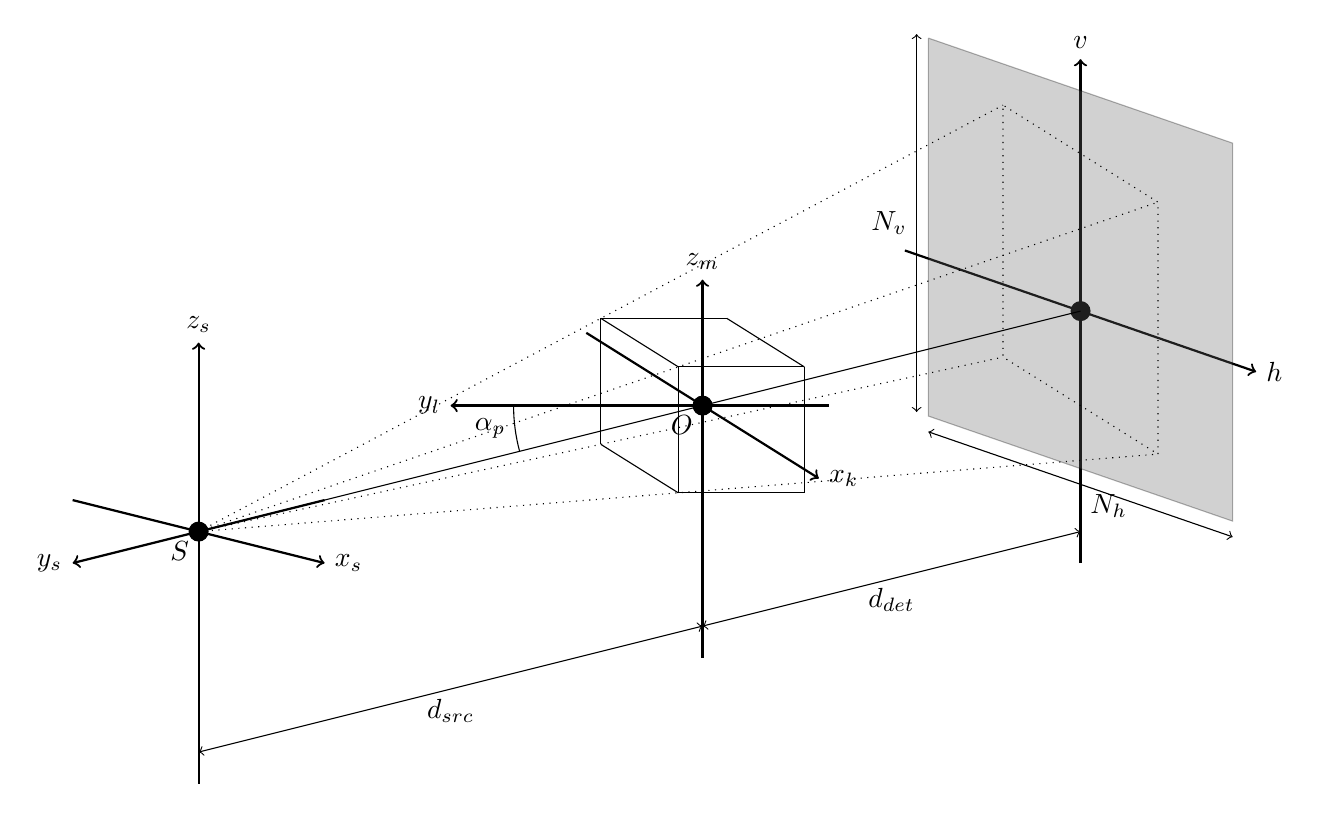
\begin{tikzpicture}[
        scale=0.8,
        axis/.style={thick,->}
    ]
    % Quelle
    \coordinate (1) at (0, 0, 0);
    \filldraw[fill=black,draw=black] (1) circle (0.15cm) node[below left] {$S$};
    \draw[axis] (-2, 0.5, 0) -- (2, -0.5, 0) node[right] {$x_s$};
    \draw[axis] (2, 0.5, 0) -- (-2, -0.5, 0) node[left] {$y_s$};
    \draw[axis] (0, -4, 0) -- (0, 3, 0) node[above] {$z_s$};

    % Volumen
    \coordinate (2) at (8, 2, 0);
    \filldraw[fill=black,draw=black] (2) circle (0.15cm) node[below left] {$O$};
    \draw[axis] (5, 2, -3) -- (11, 2, 3) node[right] {$x_k$};
    \draw[axis] (10, 2, 0) -- (4, 2, 0) node[left] {$y_l$};
    \draw[axis] (8, -2, 0) -- (8, 4, 0) node[above] {$z_m$};

    \draw (8, 1, 1) -- (10, 1, 1);
    \draw (8, 1, 1) -- (8, 3, 1);
    \draw (8, 1, 1) -- (6, 1, -1);

    \draw (8, 3, 1) -- (10, 3, 1);
    \draw (8, 3, 1) -- (6, 3, -1);

    \draw (10, 1, 1) -- (10, 3, 1);

    \draw (6, 1, -1) -- (6, 3, -1);

    \draw (6, 3, -1) -- (8, 3, -1);

    \draw (10, 3, 1) -- (8, 3, -1);


    % Detektor
    \coordinate(3) at (14, 3.5, 0);
    \filldraw[fill=black,draw=black] (3) circle (0.15cm);
    \draw[axis] (10.25, 3.5, -2.5) -- (17.75, 3.5, 2.5) node[right] {$h$};
    \draw[axis] (14, -0.5, 0) -- (14, 7.5, 0) node[above] {$v$};
    \draw[fill=black!60!white,opacity=0.3] (10.75, 7, -2.16666) -- (17.25, 7, 2.16666) -- (17.25, 1, 2.16666)
                                           -- (10.75, 1, -2.16666) -- (10.75, 7, -2.16666);
    \draw[<->] (10.5, 1, -2.33333) -- (10.5, 7, -2.33333) node[pos=0.5, left] {$N_v$};
    \draw[<->] (10.75, 0.75, -2.16666) -- (17.25, 0.75, 2.16666) node[pos=0.5, below right] {$N_h$};

    % Abstände
    \draw (1) -- (3);
    \draw[<->] (0, -3.5, 0) -- (8, -1.5, 0) node[pos=0.5,below] {$d_{src}$};
    \draw[<->] (8, -1.5, 0) -- (14, 0, 0) node[pos=0.5,below] {$d_{det}$};

    % Kegelstrahlen
    \draw[dotted] (1) -- (16, 2, 2);
    \draw[dotted] (1) -- (16, 6, 2);
    \draw[dotted] (1) -- (12, 2, -2);
    \draw[dotted] (1) -- (12, 6, -2);

    % Kegelstrahlenabbild
    \draw[dotted] (16, 2, 2) -- (16, 6, 2) -- (12, 6, -2) -- (12, 2, -2) -- (16, 2, 2);

    % Winkel
    \draw (5, 2, 0) arc (180:195:2.8cm) node[pos=0.5, left] {$\alpha_p$};
\end{tikzpicture}
\caption{Geometrie der gefilterten Rückprojektion}
\label{fig:fdk_geometrie}
\end{figure}

\subsubsection{Wichtung}\label{sssec:fdk_wichtung}

Nach der Aufnahme wird jede Projektion gewichtet. Dafür wird jedes \gls{pixel} mit den Koordinaten $(j, i)$ mit dem
Wichtungsfaktor $w_{ij}$ multipliziert.

\begin{equation}\label{eq:wichtung}
    w_{ij} = \frac{d_{det} - d_{src}}{\sqrt{(d_{det} - d_{src})^2 + h_j^2 + v_i^2}}
\end{equation}

\subsubsection{Filterung}\label{sssec:fdk_filter}

Zum Ausgleich der durch die Vorwärtsprojektion verloren gegangenen Tiefeninformationen werden die Projektionen im
nächsten Schritt zeilenweise gefiltert. Zu diesem Zweck müssen die Projektionen und der Filter allerdings mittels der
diskreten Fouriertransformation in den komplexen Raum transformiert werden; zum Einsatz kommt dabei das Verfahren der
schnellen Fouriertransformation (\textit{fast Fourier transform}, FFT) nach Cooley und Tukey~\cite{cooltuk}. Da dieses
Verfahren nur mit einer Menge von Elementen funktioniert, die einer Zweierpotenz entspricht, müssen die
Projektionszeilen und der Filter auf die nächste Zweierpotenz {\glqq}aufgerundet{\grqq} werden. Dazu wird, ausgehend von
der Länge einer Projektionszeile $N_h$,  die Filterlänge $N_{hFFT}$ berechnet:

\begin{equation}
    N_{hFFT} = 2 \cdot 2^{\left\lceil \log_{2} N_h \right\rceil}
\end{equation}

Mit der so bestimmten Filterlänge lässt sich der Filter $r$ erzeugen:

\begin{equation}\label{eq:filter_gen}
    \begin{aligned}
        r(j) \text{ mit } j &\in \left[-\frac{N_{hFFT} - 2}{2}, \frac{N_{hFFT}}{2}\right]\\
        r(j) &=
            \begin{cases}
                \frac{1}{8} \cdot \frac{1}{\tau^2} & \quad \text{wenn } j = 0\\
                0 & \quad \text{wenn } j \text{ gerade}\\
                -\frac{1}{2j^2\pi^2\tau^2} & \quad \text{wenn } j \text{ ungerade}\\
            \end{cases}
    \end{aligned}
\end{equation}

Nun wird die zu filternde Zeile so lange mit $0$ aufgefüllt, bis die erweiterte Zeile $N_{hFFT}$ \gls{pixel} umfasst:

\begin{equation}
    \begin{aligned}
        p &: \text{ mit Nullen aufgefüllte Projektionszeile}\\
        p(0 \dots N_{h - 1}) &= \text{det}(0 \dots N_{h - 1})\\
        p(N_{h} \dots N_{hFFT}) &= 0
    \end{aligned}
\end{equation}

Im Anschluss werden sowohl der Filter $r$ als auch die erweiterte Projektionszeile $p$ in den komplexen Raum
transformiert und dort miteinander multipliziert:

\begin{equation}
    \begin{aligned}
        R &= \text{FFT}(r)\\
        P &= \text{FFT}(p)\\
        F &= P \cdot R \quad \text{sowohl für den reellen als auch den imaginären Teil}
    \end{aligned}
\end{equation}

Die so gefilterte Projektionszeile $F$ wird dann mit der inversen schnellen Fouriertransformation (IFFT) in den
reellen Raum zurücktransformiert und von den {\glqq}aufgefüllten{\grqq} Elementen bereinigt:

\begin{equation}
    \begin{aligned}
        f &= \text{IFFT}(F)\\
        \text{gefilterte Projektionszeile} &: f(0 \dots N_{h - 1})
    \end{aligned}
\end{equation}

\subsubsection{Rückprojektion}

Die auf gefilterten Projektionen können nun nach dem folgenden Algorithmus für die Rückprojektion verwendet werden:

Für jede Projektion $p$ mit dem Drehwinkel $\alpha_p$:

\begin{itemize}
    \item berechne für jede \gls{voxel}koordinate $(x_k, y_l, z_m)$ deren rotierte Position $(s, t, z)$:
        \begin{equation}
            \begin{aligned}
                s &= x_k \cos \alpha_p + y_l \sin \alpha_p\\
                t &= -x_k \sin \alpha_p + y_l \cos \alpha_p\\
                z &= z_m
            \end{aligned}
        \end{equation}

    \item projiziere die rotierte \gls{voxel}koordinate $(s, t, z)$ auf den Detektor:
        \begin{equation}
            \begin{aligned}
                h' &= y' = t \cdot \frac{d_{det} - d_{src}}{s - d_{src}}\\
                v' &= z' = z \cdot \frac{d_{det} - d_{src}}{s - d_{src}}
            \end{aligned}
        \end{equation}

    \item interpoliere das Detektorsignal bei $(h', v')$:
        \begin{equation}
            \begin{aligned}
                det' = det(h', v')
            \end{aligned}
        \end{equation}

    \item führe die Rückprojektion für jedes \gls{voxel} $vol_{klm}$ aus:
        \begin{equation}
            \begin{aligned}
                vol_{klm} &= vol_{klm} + 0,5 \cdot det' \cdot u^2\\
                \text{mit } u &= \frac{d_{src}}{s - d_{src}}
            \end{aligned}
        \end{equation}
\end{itemize}

Nach Abschluss der Rückprojektion erhält man ein Volumen, dessen \gls{voxel} Aufschluss über seine innere Struktur
geben.

\subsection{Bisherige Parallelisierungsansätze}\label{ssec:par}

Aufgrund seiner geringen Komplexität und einfachen Implementierbarkeit ist der \gls{fdk} einer der beliebtesten
Rückprojektionsalgorithmen für die Kegelstrahl-Computertomographie~\cite{xumuell}. Der Vorteil des \gls{fdk} liegt
außerdem darin, dass die gefilterte Rückprojektion für jedes \gls{voxel} individuell berechnet werden kann, das heißt
ohne Abhängigkeiten zu anderen \gls{voxel}n. Dieser Umstand ermöglicht für die maschinelle Berechnung den maximalen Grad
an Parallelität, der im englischen Sprachraum auch als \textit{embarassingly parallel} bezeichnet wird, und macht den
\gls{fdk} zu einem idealen Ziel für diverse Parallelisierungsansätze. Einige neuere Ansätze sollen im Folgenden
vorgestellt werden.

Seit seiner Einführung ist der \gls{fdk} ein beliebtes Untersuchungsobjekt diverser Forschungsgruppen, die sich mit
seiner Beschleunigung bzw.\ Parallelisierung mittels einer großen Variation von Architekturen, Plattformen und
Programmiermodellen beschäftigen. 

Xu et al.\ untersuchten bereits 2004, inwieweit sich der \gls{fdk} durch den Einsatz handelsüblicher Grafikkarten
(\textit{commodity graphics hardware}) beschleunigen lässt~\cite{xumuell}. Dabei wurden die Schritte \textit{Wichtung}
und \textit{Filterung} aufgrund ihrer geringen Komplexität ($\mathcal{O}(n^2)$) auf der \gls{cpu} ausgeführt, während
man die komplexere \textit{Rückprojektion} ($\mathcal{O}(n^4)$) auf der \gls{gpu} berechnete. Die Rückprojektion fand
schichtweise statt, jeweils für eine \gls{voxel}ebene entlang der vertikalen Volumenachse. In ihrem Fazit stellten die
Autoren die Vermutung auf, dass der Abstand zwischen den Leistungen von \gls{cpu}s und \gls{gpu}s in der Zukunft
zugunsten der \gls{gpu}s immer größer werden würde: \textit{Since GPU performance has so far doubled every 6 months 
(i.e., triple of Moore's law), we expect that the gap between CPU and GPU approaches will widen even further in the near
future.}

Li et al.\ beschäftigten sich 2005 damit, wie man den \gls{fdk} mit einem \gls{fpga} implementieren könnte. Dazu teilten
sie das Ausgabevolumen, also die Zieldaten der Rückprojektion, in mehrere Würfel (\textit{bricks}) auf, um zu einer
optimalen Cachenutzung zu kommen. Der verwendete deterministische Aufteilungsalgorithmus hatte zur Folge, dass bei der
Berechnung auf dem \gls{fpga} kein Cache-Verfehlen (\textit{cache miss}) mehr auftrat.

Knaup et al.\ gingen 2007 der Frage nach, ob der \gls{fdk} durch die Eigenschaften der Cell-Architektur profitieren
könne~\cite{knaupsteck}.

Scherl et al.\ unternahmen 2008 den Versuch, den \gls{fdk} mittels \gls{cuda} zu beschleunigen~\cite{scherlkeck}. Im
Gegensatz zu der Gruppe um Xu et al.\ führten sie alle Schritte auf der \gls{gpu} aus und führten die Rückprojektion
projektionsweise durch, das heißt, dass jede Projektion einzeln in das Gesamtvolumen zurückprojiziert wurde. Diese Art
der Datenverarbeitung ermöglichte es, die Schritte \textit{Wichtung} und \textit{Filterung} parallel zur Rückprojektion
auszuführen. Zur Ausnutzung dieser Eigenschaft und zur besseren Kapselung bzw.\ Modularisierung der Teilschritte
entwickelten die Autoren daher eine Pipeline-Struktur zur parallelen Abarbeitung des Algorithmus, basierend auf dem von
Mattson et al.\ vorgestellten Entwurfsmuster~\cite{mattsan}.

Balász et al.\ versuchten 2009 das Gleiche mit der \gls{opencl}~\cite{balgab}.

Hofmann et al.\ untersuchten eventuelle Vorteile durch den Einsatz der neuen Koprozessoren vom Typ 
Intel{\textregistered} Xeon Phi{\texttrademark} {\glq}Knights Corner{\grq}~\cite{hoftrei}.

Zhao et al.\ verfolgten die Absicht, eine Beschleunigung durch Ausnutzung geometrischer Zusammenhänge zu
erreichen~\cite{zhao}. Sie setzten dabei auf die Tatsache, dass ein einmal bestimmtes, also auf den Detektor
projiziertes, \gls{voxel} durch Rotation in 90°-Schritten die rotierten \gls{voxel} ebenfalls genau bestimmt. Ist also
für ein \gls{voxel} im Projektionswinkel 0° die zugehörige Detektorkoordinate gefunden, so kann diese Detektorkoordinate
für die Projektionswinkel 90°, 180° und 270° und die entsprechenden \gls{voxel} wiederverwendet werden.

\section{Die NVIDIA{\textregistered}-CUDA{\textregistered}-Plattform}

In diesem Abschnitt wird die NVIDIA{\textregistered}-CUDA{\textregistered}-Plattform näher vorgestellt. Eingegangen wird
zunächst auf die historische Entwicklung, die die Einführung von CUDA{\textregistered} begünstigte bzw.\ erforderte. Im
Anschluss daran wird das CUDA{\textregistered}-Programmiermodell vorgestellt, das als technische Basis für die in
Kapitel~\ref{chap:umsetzung} beschriebene Implementierung dient.

\subsection{Programmierbare Grafikkarten}\label{ssec:cu_prog_gpu}

Als NVIDIA{\textregistered} im Jahre 2006 seine \textit{Compute-Unified-Device-Architecture}-Plattform
(CUDA{\textregistered}) vorstellte, die die direkte Programmierung der NVIDIA{\textregistered}-Grafikkarten ermöglichte,
folgte die Firma damit einer Entwicklung, die in den ersten Jahren des neuen Jahrtausends begonnen hatte. Mit der
Einführung der NVIDIA{\textregistered} GeForce 3 im Jahre 2001 und der parallelen Veröffentlichung von \gls{directx} 8
bzw.\ \gls{opengl} \textit{Vertex-Shader}-Erweiterungen hatten Anwendungsentwickler erstmals Zugriff auf die
\textit{Shader}-Einheiten für die \textit{Vertex}- und \textit{Transform-\&-Lighting}-Berechnung. Spätere \gls{gpu}s,
die mit \gls{directx} 9 kompatibel waren, gestatteten eine noch flexiblere Programmierung, indem sie Entwicklern Zugriff
auf die \textit{Pixel-Shader} erlaubten und die Nutzung von Texturen im \textit{Vertex-Shader} zuließen. Die 2002
vorgestellte \gls{gpu} ATI Radeon 9700 verfügte über einen programmierbaren
24bit-Fließkommazahl-\textit{Pixel-Shader}-Prozessor, der mit \gls{directx} 9 und \gls{opengl} gesteuert werden
konnte, die GeForce{\textregistered} FX bot sogar 32bit-Fließkommazahl-Pixel-Prozessoren. Diese programmierbaren
Prozessoren waren Teil einer Entwicklung, die zu einer allmählichen Vereinheitlichung der auf der \gls{gpu} verbauten
Funktionseinheiten führte: während es auf den GeForce{\textregistered}-Serien 6800 und 7800 noch getrennte Prozessoren
für die \textit{Vertex}- und \textit{Pixel}-Berechnung gab, wurde in der 2005 erschienenen XBox 360 eine 
{\glqq}vereinheitlichte{\grqq} Grafikkarte verbaut, deren Prozessoreinheiten sowohl für die \textit{Vertex}- als auch
für die \textit{Pixel}-Berechnung geeignet waren (vgl.~\cite{kirkhwu}, S. 28 -- 29).

Durch diese Vereinheitlichung der \gls{gpu}-Prozessoren glich die Hardware mehr und mehr den aus dem \gls{hpc} bekannten
Parallelrechnern. Mit der Verfügbarkeit \gls{directx}-9-kompatibler \gls{gpu}s wurde diese Entwicklung zunehmend
auch in Forschungskreisen bekannt und man begann zu untersuchen, inwiefern sich die neue Hardware zur Lösung von
berechnungsintensiven Problemen aus den Bereichen der Natur- und Ingenieurswissenschaften einsetzen ließ. Die zu diesen
Zwecken nicht konstruierten \gls{gpu}s ließen sich jedoch nur über die vorhandenen Schnittstellen zur
Grafikprogrammierung ansteuern. Zur Nutzung der Hardwareressourcen musste ein Programmierer daher das zu lösende Problem
zunächst auf computergrafische Operationen abbilden, sodass die Berechnung dann mit \gls{opengl} oder \gls{directx}
durchgeführt werden konnte. Um beispielsweise eine mathematische Funktion mehrfach auszuführen, musste diese erst in
ein \textit{Pixel-Shader}-Programm umgeschrieben werden, während die zugehörigen Eingabedaten als Texturen
vorzuliegen hatten und die Ausgabedaten im der jeweiligen Grafikbibliothek eigenen Pixelformat zurückgegeben wurden.
Die Umschreibung in einen für die Verwendung von \textit{Pixel-Shadern} geeigneten Algorithmus hatte außerdem den
gravierenden Nachteil, dass Zugriffe auf beliebige Stellen im Speicher nicht möglich waren. Da ein \textit{Pixel-Shader}
als Ausgabedatum die Farbe eines \gls{pixel}s zurückliefert, besteht dazu aus Sicht der Grafikbibliothek auch keine
Notwendigkeit, da die Position des zugehörigen Pixels ja bereits bekannt ist (vgl.~\cite{kirkhwu}, S. 33).

Diese Beschränkungen erwiesen sich für generische numerische Berechnungen bald als zu restriktiv. Erschwerend kam hinzu, 
dass jeder Entwickler, der sich mit diesen technischen Limitierungen abfinden konnte, zusätzlich noch Wissen über die
Funktionsweise von \gls{opengl} und \gls{directx} benötigte, um das zu lösende Problem mit Hilfe von \gls{gpu}s
bewältigen zu lassen. Eine flächendeckende Akzeptanz von \gls{gpu}s als Beschleunigern war unter Forschern daher in den
ersten Jahren des \gls{gpgpu} nicht gegeben (vgl.~\cite{sandkand}, S. 6).

Die Situation änderte sich, als NVIDIA{\textregistered} 2006 die GeForce{\textregistered} 8800 GTX der Öffentlichkeit
präsentierte. Diese \gls{gpu} war nicht nur zum damals neuen \gls{directx} 10 kompatibel, sondern auch die erste
Grafikkarte, die mit \gls{cuda} ohne den Umweg über \gls{directx} oder \gls{opengl} direkt programmierbar war
(vgl.~\cite{sandkand}, S. 7). Programmierer hatten nun die Möglichkeit, \textit{datenparallele} Aspekte
(vgl. Abschnitt~\ref{sssec:cu_data_par}) des zu lösenden Problems zu deklarieren und von der \gls{gpu} ausführen zu
lassen. Die \textit{Shader}-Prozessoren hatten sich zu komplett programmierbaren Prozessoren entwickelt und verfügten
über einen Instruktionsspeicher, einen Instruktions-Cache und eine Instruktionskontrollogik. Diesen zusätzlichen
Hardwareoverhead konnte NVIDIA{\textregistered} dadurch reduzieren, dass mehrere Prozessoren sich den Instruktionscache
und die -kontrolllogik teilten. Diese Struktur funktioniert aufgrund des Hardware-Fokus auf die parallele Berechnung von
\gls{pixel}n für \gls{gpu}s gut. Zusätzlich war es nun möglich, auf beliebige Teile des Speichers zuzugreifen. Aus Sicht
des Entwicklers lag nun ein Programmiermodell vor, das eine Hierarchie paralleler Threads, Synchronisierungsmechanismen
und Barrieren sowie atomare Operationen bot und das Ganze in eine an C bzw.\ C++ angelehnte Sprache einbettete
(vgl.~\cite{kirkhwu}, S. 35).

\subsection{Das \gls{cuda}-Programmiermodell}

In diesem Abschnitt wird das der \gls{cuda}-Plattform zugrundeliegende Programmiermodell näher vorgestellt. Das
gedankliche Fundament dieses Modell ist die \textit{Datenparallelität}, die in Abschnitt~\ref{sssec:cu_data_par}
erläutert wird. Die konkreten Programmierkonzepte schließen sich in den danach folgenden Abschnitten an.

\subsubsection{Datenparallelität}\label{sssec:cu_data_par}

Moderne Programme bearbeiten häufig große Datenmengen und benötigen deswegen auf herkömmlichen Rechnern lange
Ausführungszeiten. Viele Anwendungen arbeiten dabei mit Daten, die Vorgänge der echten Welt ab- oder nachbilden, wie
beispielsweise einfache Bilder oder Filme oder die Bewegungen von Flüssigkeiten und Gasen unter bestimmten Umständen.
Fluglinien müssen ihre Flüge planen, wozu die Daten einer Vielzahl anderer Flüge, Besatzungen und Flughäfen herangezogen
werden, die voneinander unabhängig sind. Diese Unabhängigkeit der Daten ist die Voraussetzung für datenparallele
Algorithmen.

Als einfaches Beispiel für einen datenparallelen Algorithmus lässt sich die Addition zweier Vektoren $A$ und $B$
betrachten:

\begin{equation*}
    \left(
        \begin{array}{c}
            a_1\\
            a_2\\
            a_3
        \end{array}
    \right)
    +
    \left(
        \begin{array}{c}
            b_1\\
            b_2\\
            b_3
        \end{array}
    \right)
    =
    \left(
        \begin{array}{c}
            a_1 + b_1 \\
            a_2 + b_2 \\
            a_3 + b_3
        \end{array}
    \right)
    =
    \left(
        \begin{array}{c}
            c_1 \\
            c_2 \\
            c_3
        \end{array}
    \right)
\end{equation*}

In diesem Beispiel wird $c_1$ berechnet, indem $a_1$ und $b_1$ addiert werden, und $c_3$ ergibt sich aus der Addition
von $a_3$ und $b_3$. Die Additionen sind voneinander unabhängig und können parallel berechnet werden. Sehr große
Vektoren führen in diesem Beispiel daher zu einem hohen Maß an Datenparallelität.

Der Datenparallelität steht das Konzept der \textit{Task-Parallelität} gegenüber. Die Task-Parallelität kommt vor allem
in komplexeren Programmen zur Anwendung, in denen es mehrere unterschiedliche Aufgaben gibt, die parallel bearbeitet
werden können. Vorstellbar ist z.B.\ ein Programm zur Filterung von Bildern, in denen ein Task das die Bilder
nacheinander lädt, der zweite die Bilder nacheinander filtert und ein weiterer die gefilterten Bilder wieder
abspeichert (vgl.~\cite{kirkhwu}, S. 42 -- 43).

\subsubsection{Parallele Ausführung}

Die Ausführung eines \gls{cuda}-Programms beginnt auf dem \gls{host}. Wird ein \gls{kernel} aufgerufen, so wird auf dem
\gls{device} eine Anzahl an Threads gestartet. Die Summe aller auf dem \gls{device} gestrateten Threads bezeichnet
man als \textit{\gls{grid}}. Haben alle Threads eines \gls{kernel}s ihre Ausführung beendet, wird auch das \gls{grid}
beendet.
Das Starten eines \gls{kernel}s erzeugt typischerweise eine große Zahl von Threads. Im Gegensatz zur \gls{cpu}, auf der
das Erzeugen eines Threads in der Regel mehrere tausend Takte benötigt, ist der gleiche Vorgang auf der \gls{gpu} in
einigen wenigen Takten zu bewältigen (vgl.~\cite{kirkhwu}, S. 44 -- 45).

Das Beispiel der Vektoraddition aus Abschnitt~\ref{sssec:cu_data_par} lässt sich in C++ wie in
Quelltext~\ref{source:vec_add_cpp} dargestellt implementieren. 

\begin{code}
\begin{minted}[breaklines,breakafter=\,,fontsize=\small]{c++}
auto vec_add(const std::int32_t* A, const std::int32_t* B,
             std::int32_t* C, std::size_t size) -> void
{
    for(auto i = 0u; i < size; ++i)
        C[i] = A[i] + B[i];
}
\end{minted}
\captionof{listing}{Vektoraddition mit C++}
\label{source:vec_add_cpp}
\end{code}

In \gls{cuda} würde dagegen jeder Thread ein Element des Ausgabevektors $C$ berechnen, wie in
Quelltext~\ref{source:vec_add_cuda} gezeigt.

\begin{code}
\begin{minted}[breaklines,breakafter=\,,fontsize=\small]{cuda}
__global__ void vec_add(const std::int32_t* A, const std::int32_t* B,
                        std::int32_t* C, std::size_t size)
{
    auto i = blockIdx.x * blockDim.x + threadIdx.x;
    if(i < size)
        C[i] = A[i] + B[i];
}
\end{minted}
\captionof{listing}{Vektoraddition mit \gls{cuda}}
\label{source:vec_add_cuda}
\end{code}

Die Berechnung der Indices erfolgt in diesem Beispiel nicht über eine fortlaufend inkrementierte Variable, wie es in C++
der Fall wäre, sondern über die Hilfsvariablen \texttt{blockIdx}, \texttt{blockDim} und \texttt{threadIdx}. Wird ein
\gls{cuda}-\gls{kernel} ausgeführt, so entsteht auf dem \gls{device} ein Thread-\gls{grid}. Diese Threads werden in
einer zweistufigen Hierarchie angeordnet. Jedes \gls{grid} besteht aus mehreren Thread-Blöcken, die der Einfachheit
halber in der Folge als \textit{Blöcke} bezeichnet werden. Alle Blöcke innerhalb eines \gls{grid}s haben die gleiche
Größe, können jedoch maximal 1024 Threads umfassen; die Thread-Zahl der Blöcke wird auf dem \gls{host} vor der
Ausführung des \gls{kernel}s definiert. Für ein gegebenes \gls{grid} kann die Anzahl der Threads pro Block durch die 
Variable \texttt{blockDim} abgefragt werden, während der individuelle Block, zu dem ein bestimmter Thread gehört, durch
die Variable \texttt{blockIdx} identifiert werden kann. Innerhalb eines Blocks kann ein einzelner Thread über die
Variable \texttt{threadIdx} bestimmt werden. Für den ersten Thread des Blocks \texttt{0} hat \texttt{threadIdx} also den
Wert \texttt{0}, für den zweiten \texttt{1}, für den dritten \texttt{2}, usw. Durch die Kombination der drei Variablen,
wie sie in Quelltext~\ref{source:vec_add_cuda} dargestellt ist, lässt sich somit jeder Thread innerhalb des \gls{grid}s
eindeutig identifizieren. Da \gls{cuda} das Starten von zwei- und dreidimensionalen \gls{kernel}n unterstützt, kann über
die Felder \texttt{x}, \texttt{y} und \texttt{z} die Zahl der Blöcke bzw.\ Threads in der jeweiligen Dimension bestimmt
werden (vgl.~\cite{kirkhwu}, S. 54).

Ein weiterer Unterschied zur herkömmlichen C++-Programmierung ist das Schlüsselwort \texttt{\_\_global\_\_} vor der
Deklaration. Dieses Schlüsselwort dient zur Identifizierung einer Funktion als \gls{kernel}, also einer Funktion auf
dem \gls{device}, die vom \gls{host} aus aufgerufen werden kann. Daneben verwendet \gls{cuda} die Schlüsselworte
\texttt{\_\_device\_\_} und \texttt{\_\_host\_\_}, die anzeigen, auf welcher Hardware die jeweilige Funktion ausgeführt
werden kann bzw.\ soll. Eine \texttt{\_\_device\_\_}-Funktion kann dabei nur innerhalb eines \gls{kernel}s oder einer
weiteren \texttt{\_\_device\_\_}-Funktion aufgerufen werden, eine \texttt{\_\_host\_\_}-Funktion nur auf dem \gls{host}
-- sie entspricht also einer normalen C++-Funktion (vgl. Tabelle~\ref{table:cu_func_keywords} und~\cite{kirkhwu}, S.55).

\begin{table}
    \centering
    \begin{tabular}{| l | c | c |}
        \hline
        & Ausgeführt auf dem & Aufgerufen vom \\
        \hline
        \texttt{\_\_device\_\_ float device\_func()} & \gls{device} & \gls{device} \\
        \hline
        \texttt{\_\_global\_\_ void kernel\_func()} & \gls{device} & \gls{host} \\
        \hline
        \texttt{\_\_host\_\_ float host\_func()} & \gls{host} & \gls{host} \\
        \hline
    \end{tabular}
    \caption{\gls{cuda}-Schlüsselworte für die Funktionsdeklaration}
    \label{table:cu_func_keywords}
\end{table}

\subsubsection{Architektur}\label{sssec:cu_arch}

\subsubsection{Speicher}\label{sssec:cu_mem}

\subsubsection{\glspl{stream}}\label{sssec:cu_streams}
